%!LW recipe=latexmk (lualatex)
%Use lualatex to compile
%Therefore, do not use amssymb, input/output enc
% Get \@ doesn't match definition? Try deleting all auxillary files.
\DocumentMetadata{
 lang=en,
 testphase={phase-III,math,table,title,firstaid},
 pdfversion=2.0,
 pdfstandard=ua-2,
 pdfstandard=a-4f,
 uncompress
}
\documentclass[11pt]{isuthesistagged}
%Command below can toggle off tagging,
%speeding up compiling during drafting stages
%Comment out when ready to submit
%\tagpdfsetup{activate/all=false}

%Caption package & tagging fixes
\usepackage{caption}
%This work-around comes from: https://github.com/latex3/tagging-project/issues/720
\RemoveFromHook{begindocument}[latex-lab-testphase-float]
\makeatletter
\ExplSyntaxOn
\socket_new_plug:nnn{tagsupport/parbox/before}{caption}
  {   
   \tagpdfparaOn %restart para tagging
   \tl_if_empty:NTF\@current@float@struct
    {     
     \tag_struct_begin:n{tag=Caption,firstkid}
    }
    {
     \tag_struct_begin:n{tag=Caption,parent=\@current@float@struct,firstkid}
    } 
  }
\socket_new_plug:nnn{tagsupport/parbox/after}{caption}
  {
   \tag_struct_end:   
  }
\l@addto@macro\caption@beginex@hook{%
  \tagpdfparaOff %leavevmode in parbox should not start paragraph structure
  \AssignSocketPlug{tagsupport/parbox/before}{caption}
  \AssignSocketPlug{tagsupport/parbox/after}{caption}}
\ExplSyntaxOff
\AtBeginDocument{
	\renewcommand*\caption@anchor[1]{%
        \ifmeasuring@ \else
           \caption@raisedlink{\MakeLinkTarget*{#1}}%
        \fi}%  
}
\makeatother

%%Mathy packages
\usepackage{amsmath}
\usepackage{amsthm}
\usepackage{mathrsfs}
\usepackage{bm}
\usepackage{mathtools}
\usepackage{thmtools}
\usepackage{templatedShortcuts-private}
%%
\usepackage[default]{fontsetup}

\usepackage{unicode-math}

\usepackage{graphicx}

\chaptertitle
% Old-style, thesis numbering down to subsubsection
\alternate
\usepackage{rotating}
% Bibliography without numbers or labels
%Natbib compatibility mode activated
%Different styles available - look at biblatex documentation
\usepackage[natbib=true,style=authoryear,style=apa]{biblatex}
\addbibresource{thesisAccessTest.bib}
\setlength{\bibitemsep}{13.2pt}

%Set the author
\newcommand{\theAuthor}{Alice Wonder}
%Set the tite 
\twoLineTitle{This is the title of the thesis
submitted to Iowa State University on the first line}{
Note that only the first letter of
the first word and proper names
are capitalized and this is the second line}

%%PDF properties automatically set
\author{\theAuthor}
\title{\titleWithLineBreak}
\usepackage[hypertexnames=false,linktocpage=true,pdfauthor={\theAuthor},pdftitle={\titleWithoutBreak},]{hyperref}
\hypersetup{colorlinks=true,linkcolor=blue,citecolor=blue,filecolor=blue,urlcolor=blue,bookmarksnumbered=true,pdfview=FitB,pdfencoding=auto}
\usepackage{bookmark}
% The following piece of code removes extra space on the top of each chapter
%  that is default of latex report class documents

\usepackage{etoolbox}
\makeatletter
\setlength{\@fptop}{0pt} %command added to ensure images always float on top of the page
\makeatother

%%%%%%%%%%%%%%%%%%%%%%%%%%%
\usepackage{float}
%%%%%%%%%%%%%%%%%%%%%%%%%%%%%%%%%%
\usepackage{xcolor}
\usepackage{graphicx}
\usepackage{geometry}
\geometry{letterpaper, left=1in, top=1in, right=1in, bottom=1in, includehead=true,headheight=14pt} 
\usepackage{pdflscape}
%%%%%%%%%%%%%%%%%%%%%%%%%%%%%%%%%%

\usepackage[intoc, english]{nomencl}
\doublespacing
\AtBeginEnvironment{table}{\singlespacing}% 
\AtBeginEnvironment{figure}{\singlespacing}% 

%%%Captioning Format
\DeclareCaptionListFormat{figureList}{Figure #1#2}
\DeclareCaptionListFormat{tableList}{Table #1#2}
\captionsetup[figure]{listformat=figureList}
\captionsetup[table]{listformat=tableList}
\captionsetup[ContinuedFloat]{list=no}


\usepackage[inline]{enumitem}


%Gets rid of footnote rule(line)
%\renewcommand*\footnoterule{}

\begin{document}
\DeclareGraphicsExtensions{.jpg,.pdf,.mps,.png}
%\begin{singlespace}
\def\@makechapterheada{\vspace*{-2cm}\titlepage} % in order to reduce the space between margin and heading in titlepage
% Template Titlepage File
% Please choose appropriate options for Master's thesis, Doctoral dissertations, and creative components. Please read the comments to make an informed choice

\@makechapterheada\titlepage  % using definition from thesis.tex reduce the space between margin and heading in titlepage
\title{\theTitle}

\author{\theAuthor}

%%%%%%%%%%%%%%%%%%%

\degree{DOCTOR OF PHILOSOPHY}
\major{Mathematics}

\level{doctoral}
\mprof{John Smith}
% In case of co majors please comment out the mprof line above and use the following two lines of mprofs and cmprofs to defines the two co-major profs
%\mprofs{ABC}
%\cmprofs{DEF}

\format{dissertation}
\committee{4}
\members{Jane Dee \\ Allen Wrench}
\disclaimertitlepage{The student author, whose presentation of the scholarship herein was approved by the program of study committee, is solely responsible for the content of this dissertation. The Graduate College will ensure this dissertation is globally accessible and will not permit alterations after a degree is conferred.}


%%%%%%%%%%%%%%%%%%%%%%%%%%%%
% Doctor of Philosophy options
% If co-majors select only co-major options as described and skip other options like \major, \mprof and make sure committee members are appropriately included.


% Add these additional lines for a Doctoral Dissertation
%\degree{DOCTOR OF PHILOSOPHY}
% \major{Human Development and Family Studies (Marriage and Family Therapy)}
% Use the following line for co-majors (usually used with doctoral dissertations)
%\comajors{Statistics; Computer Science}{}
%\level{doctoral}
%\mprof{Susan D. Ross}
% In case of co majors please comment out the mprof line above and use the following two lines of mprofs and cmprofs to defines the two co-major profs
%\mprofs{ABC}
%\cmprofs{DEF}

%\format{dissertation}
%\committee{4}
%\members{Mary Jones \\ Bjork Petersen \\ Sam Anders \\ Harold Jones}
%\disclaimertitlepage{The student author, whose presentation of the scholarship herein was approved by the program of study committee, is solely responsible for the content of this dissertation/thesis. The Graduate College will ensure this dissertation/thesis is globally accessible and will not permit alterations after a degree is conferred.}

%%%%%%%%%%%%%%
% Creative component: lines to add / remove
% Add these additional lines for a Creative Component
% - also comment out the \maketitle command
%\format{Creative Component}
%\submit{the graduate faculty}

\notice
\maketitle

\fancypagestyle{plain}{}


% % Left-justified setting for all sections including
% % dedication, nomenclature, acknowledgement, abstract and all chapters
% % Re-position the two lines below will change all the section
% % being compiled after those two lines
\raggedright
\parindent 0.25 in % set all paragraphs in the document to have indent
% %%%%%%%%%%%%%%%%%%%%%%%%%%%%%%%%%%%%%%%%%
% %% The line below adds the word "Page" over the page numbers in TOC, LOT, LOF
\addtocontents{toc}{~\hfill\tagstructbegin{tag=H2,stash,label=pageOfTOC}\tagmcbegin{tag=H2}\textbf{Page}\par\tagmcend\tagstructend}
\addtocontents{lot}{~\hfill\tagstructbegin{tag=H2,stash,label=pageOfLOT}\tagmcbegin{tag=H2}\textbf{Page}\par\tagmcend\tagstructend}
\addtocontents{lof}{~\hfill\tagstructbegin{tag=H2,stash,label=pageOfLOF}\tagmcbegin{tag=H2}\textbf{Page}\par\tagmcend\tagstructend}

% %%
% % Optional thesis dedication
%   Dedication is not usually listed in the table of contents.
%   However, if you do want it, add this command here (not in the dedication file)
%   \addToBibWithoutChapter{DEDICATION}
\chapter*{DEDICATION}

I would like to dedicate this thesis to my wife Glenda and
to my daughter Alice without whose support I would not have
been able to complete this work.



% % Table of Contents, List of Tables and List of Figures

{
\pdfbookmark[0]{TABLE OF CONTENTS}{table}
\tableofcontents
\tagstructuse{pageOfTOC} %gets tagging of "Page" done
}

\addtocontents{toc}{\def\protect\@chapapp{}} \cleardoublepage \phantomsection
\pagebreak
% %%%%%%%%%%%%%%%%%%%%%%%%%%%%%%%%%%%%%%%%%
\MakeLinkTarget[specialchapter]{}%necessary for tagging (as of 2024)
\addcontentsline{toc}{chapter}{LIST OF TABLES}
\listoftables
\tagstructuse{pageOfLOT}%gets tagging of "Page" done
% %%%%%%%%%%%%%%%%%%%%%%%%%%%%%%%%%%%%%%%%%
\cleardoublepage \phantomsection
\MakeLinkTarget[specialchapter]{} %necessary for tagging (as of 2024)
\addcontentsline{toc}{chapter}{LIST OF FIGURES}
\listoffigures
\tagstructuse{pageOfLOF}%gets tagging of "Page" done
% %%%%%%%%%%%%%%%%%%%%%%%%%%%%%%%%%%%%%%%%%


% %Optional Nomenclature
\cleardoublepage \phantomsection
\MakeLinkTarget[specialchapter]{}
\makenomenclature
\renewcommand{\nomname}{NOMENCLATURE}
%\specialchapt{NOMENCLATURE}

%\mbox{}
\renewcommand\nomgroup[1]{%
  \item[\bfseries
  \ifstrequal{#1}{P}{Physics Constants}{%
  \ifstrequal{#1}{N}{Number Sets}{%
  \ifstrequal{#1}{O}{Other Symbols}{}}}%
]}

\nomenclature[P]{$c$}{Speed of light in a vacuum inertial system}
\nomenclature[P]{$h$}{Plank Constant}
\nomenclature[P]{$g$}{Gravitational Constant}
\nomenclature[N]{$\mathbb{R}$}{Real Numbers}
\nomenclature[N]{$\mathbb{C}$}{Complex Numbers}
\nomenclature[N]{$\mathbb{H}$}{Quaternions}
\nomenclature[O]{$V$}{Constant Volume}
\nomenclature[O]{$\rho$}{Friction Index}

\renewcommand{\nompreamble}{The nomenclature for your dissertation or thesis is optional. This list may be placed in
the following places: as the last preliminary page, before the Reference section, or as an Appendix. The heading is bold if other major headings are bold, and the list is in the same font size and style as text. Nomenclature should follow a two-column format with the term in the left
column and its definition or description within the right column.}

\printnomenclature

% The following link has more tweaks, tips and tricks on how to setup nomenclatures: https://www.overleaf.com/learn/latex/Nomenclatures

%Adds Chapter in front of chapter on TOC
\addtocontents{toc}{\def\protect\@chapapp{CHAPTER\ }}


%Optional Acknowledgements
\cleardoublepage \phantomsection
\specialchapt{ACKNOWLEDGMENTS}

I would like to take this opportunity to express my thanks to those
who helped me with various aspects of conducting research and the writing
of this thesis.
First and foremost, Dr. Susan D. Ross for her guidance, patience and support
throughout this research and the writing of this thesis.
Her insights and words of encouragement have often inspired me and renewed
my hopes for completing my graduate education.
I would also like to thank my committee members for their efforts
and contributions to this work: Dr. August Tanner and
Dr. Lewis Hargrave.
I would additionally like to thank
Dr. Tanner for his guidance throughout the initial stages of my
graduate career and Dr. Hargrave for his inspirational teaching style.

%Optional thesis abstract
\cleardoublepage \phantomsection
\specialchapt{ABSTRACT}

This is the text of my abstract that is part of the thesis itself.
The abstract describes the work in general and the heading and style
match the rest of the document.

\cleardoublepage \phantomsection

\newpage
\pagenumbering{arabic}
\pagestyle{fancy}
% Chapter 1 of the Thesis Template File
\chapter{OVERVIEW}

This is the opening paragraph to my thesis which
explains in general terms the concepts and hypothesis
which will be used in my thesis.

With more general information given here than really
necessary.

\section{Introduction} \label{introSection}

Here initial concepts and conditions are explained and several hypothesis are mentioned in brief.

\subsection{Hypothesis}

Here one particular hypothesis is explained in depth and is examined in the light of current literature.

\subsubsection{Parts of the hypothesis}

Here one particular part of the hypothesis that is 
currently being explained is examined and particular
elements of that part are given careful scrutiny.

% Below \subsubsection
% Sectional commands: \paragraph and \subparagraph may also be used

\subsection{Second Hypothesis}

Here one particular hypothesis is explained in depth
and is examined in the light of current literature.

\subsubsection{Parts of the second hypothesis}

Here one particular part of the hypothesis that is 
currently being explained is examined and particular
elements of that part are given careful scrutiny.

\section{Criteria Review}

Here certain criteria are explained thus eventually
leading to a foregone conclusion.



\autocite{correaValadierlikeFormulasSupremum},\autocite{kleeHellyTheoremIts1963}

% Chapter 2 of the Thesis Template File
%   which includes bibliographic references.
\chapter{REVIEW OF LITERATURE}

This is the opening paragraph to my thesis which
explains in general terms the concepts and hypothesis
which will be used in my thesis.

With more general information given here than really
necessary.

\section{Introduction}

Here initial concepts and conditions are explained and
several hypothesis are mentioned in brief.

did the initial work in this area. But in Struss' work \autocite{buiEveryGeneratingPolytope2023}
the definitive model is seen.

\subsection{Hypothesis}

Here one particular hypothesis is explained in depth
and is examined in the light of current literature.

\subsubsection{Parts of the hypothesis}

Here one particular part of the hypothesis that is
currently being explained is examined and particular
elements of that part are given careful scrutiny.

% Below \subsubsection
% Sectional commands: \paragraph and \subparagraph may also be used

\subsection{Second Hypothesis}

\paragraph{Heading} Here one particular hypothesis is explained in depth
and is examined in the light of current literature. \subparagraph{Even smaller heading} Another sentence.

\subsubsection{Parts of the second hypothesis}

Here one particular part of the hypothesis that is
currently being explained is examined and particular
elements of that part are given careful scrutiny.

\section{Criteria Review}

Here certain criteria are explained thus eventually
leading to a foregone conclusion.
\section{Continuing Tables}
Note, tables with cells spanning multiple columns work automatically, but cells spanning multiple rows require extra tagging.
\begin{table}[ht]
    \caption{This is a two-part table that also has cells spanning multiple rows.}
    %use \tagpdfsetup{table/tagging=presentation} if and only if the table
    %is for alignment/presentation purposes and is not a real table
    %
    %\tagpdfsetup{table/header-rows={1,2}} would have rows 1 and 2 be header rows
    \tagpdfsetup{table/header-rows={1}}
    %Use \tagpdfsetup{table/header-columns={}} for header columns instead
    %Put \tagpdfsetup{table/multirow={⟨number of rows⟩}} in cells spanning multiple rows
    %Note, multicolumn works automatically (no extra commands necessary)
    \begin{tabular}{rrrlrrrr}
        k      & q          & p+ & p- & s1                                                         & s2                                                         & s3                                                         & RHS       \\ \hline
        2      & 2          & 2  & 1  & 1                                                          & 0                                                          & 0                                                          & 1         \\
        -T     & 0          & 1  & 1  & 0                                                          & 1                                                          & 0                                                          & 0         \\
        T      & -1         & 0  & 1  & 0                                                          & 0                                                          & 1                                                          & 0         \\
        -1     & 1          & -1 & 1  &                                                            &                                                            &                                                            &           \\ \hline
        2(T+1) & 2          & 0  & 1  & 1                                                          & -2                                                         & 0                                                          & 1         \\ \hline
        -T     & 0          & 1  & 1  & 0                                                          & 1                                                          & 0                                                          & 0         \\
        T      & -1         & 0  & 1  & 0                                                          & 0                                                          & 1                                                          & 0         \\
        -(T+1) & 1          & 0  & 1  & 0                                                          & 1                                                          & 0                                                          &           \\ \hline
        0      & 2+2(T+1)/T & 0  & 1  & 1                                                          & -2                                                         & -2(T+1)/T                                                  & 1         \\ \hline
        0      & -1         & 1  & 1  & 0                                                          & 1                                                          & 1                                                          & 0         \\
        1      & -1/T       & 0  & 1  & 0                                                          & 0                                                          & 1/T                                                        & 0         \\
        0      & 1-(T+1)/T  & 0  & 1  & 0                                                          & 1                                                          & (T+1)/T                                                    &           \\ \hline
        0      & 2(2T+1)/T  & 0  & 1  & 1                                                          & -2                                                         & -2(T+1)/T                                                  & 1         \\ \hline
        0      & -1         & 1  & 1  & 0                                                          & 1                                                          & 1                                                          & 0         \\
        1      & -1/T       & 0  & 1  & 0                                                          & 0                                                          & 1/T                                                        & 0         \\
        0      & -1/T       & 0  & 1  & 0                                                          & 1                                                          & (T+1)/T                                                    &           \\ \hline
        0      & 1          & 0  & 1  & T/2(2T+1)                                                  & -T/(2T+1)                                                  & -1                                                         & T/2(2T+1) \\ \hline
        0      & 0          & 1  & 1  & T/2(2T+1)                                                  & 1-T/(2T+1)                                                 & 0                                                          & T/2(2T+1) \\
        1      & 0          & 0  & 1  & 1/2(2T+1)                                                  & -1/(2T+1)                                                  & 0                                                          & 1/2(2T+1) \\ \hline
        0      & 0          & 0  & 1  & 1/2(2T+1)                                                  & 1-1/(2T+1)                                                 & -1+(T+1)/TT                                                &           \\ \hline
        0      & 0          & 0  & 1  & 1/2(2T+1)                                                  & 1-1/(2T+1)                                                 & -1+(T+1)/TT                                                &           \\ \hline
        0      & 0          & 0  & 0  & \tagpdfsetup{table/multirow={8}}\multirow{8}{*}{1/2(2T+1)} & \tagpdfsetup{table/multirow={8}}\multirow{8}{*}{1/2(2T+1)} & \tagpdfsetup{table/multirow={8}}\multirow{8}{*}{1/2(2T+1)} &           \\ \cline{1-4}
        0      & 0          & 0  & 0  &                                                            &                                                            &                                                            &           \\ \cline{1-4}
        0      & 0          & 0  & 0  &                                                            &                                                            &                                                            &           \\ \cline{1-4}
        0      & 0          & 0  & 0  &                                                            &                                                            &                                                            &           \\ \cline{1-4}
        0      & 0          & 0  & 0  &                                                            &                                                            &                                                            &           \\ \cline{1-4}
        0      & 0          & 0  & 0  &                                                            &                                                            &                                                            &           \\ \cline{1-4}
        0      & 0          & 0  & 0  &                                                            &                                                            &                                                            &           \\ \cline{1-4}
        0      & 0          & 0  & 0  &                                                            &                                                            &                                                            &           \\ \hline
    \end{tabular}
\end{table}
%\tagpdfsetup{table/header-rows={1,2}} would have rows 1 and 2 be header rows
\tagpdfsetup{table/header-rows={1}}
%Use \tagpdfsetup{table/header-columns={}} for header columns instead
%Put \tagpdfsetup{table/multirow={⟨number of rows comma separated ⟩} in cells spanning multiple rows
\begin{table}[ht]
    %As a continued table, use \ContinuedFloat to keep the same #
    %And use the text "Continued" inside the caption
    \ContinuedFloat
    \caption{Continued}
    %\tagpdfsetup{table/header-rows={1,2}} would have rows 1 and 2 be header rows
    \tagpdfsetup{table/header-rows={1}}
    %Use \tagpdfsetup{table/header-columns={}} for header columns instead
    %Put \tagpdfsetup{table/multirow={⟨number of rows comma separated ⟩} in cells spanning multiple rows

    \begin{tabular}{rrrlrrrr}
        k      & q          & p+ & p- & s1        & s2         & s3          & RHS       \\ \hline
        2      & 2          & 2  & 1  & 1         & 0          & 0           & 1         \\
        -T     & 0          & 1  & 1  & 0         & 1          & 0           & 0         \\
        T      & -1         & 0  & 1  & 0         & 0          & 1           & 0         \\
        -1     & 1          & -1 & 1  &           &            &             &           \\ \hline
        2(T+1) & 2          & 0  & 1  & 1         & -2         & 0           & 1         \\ \hline
        -T     & 0          & 1  & 1  & 0         & 1          & 0           & 0         \\
        T      & -1         & 0  & 1  & 0         & 0          & 1           & 0         \\
        -(T+1) & 1          & 0  & 1  & 0         & 1          & 0           &           \\ \hline
        0      & 2+2(T+1)/T & 0  & 1  & 1         & -2         & -2(T+1)/T   & 1         \\ \hline
        0      & -1         & 1  & 1  & 0         & 1          & 1           & 0         \\
        1      & -1/T       & 0  & 1  & 0         & 0          & 1/T         & 0         \\
        0      & 1-(T+1)/T  & 0  & 1  & 0         & 1          & (T+1)/T     &           \\ \hline
        0      & 2(2T+1)/T  & 0  & 1  & 1         & -2         & -2(T+1)/T   & 1         \\ \hline
        0      & -1         & 1  & 1  & 0         & 1          & 1           & 0         \\
        1      & -1/T       & 0  & 1  & 0         & 0          & 1/T         & 0         \\
        0      & -1/T       & 0  & 1  & 0         & 1          & (T+1)/T     &           \\ \hline
        0      & 1          & 0  & 1  & T/2(2T+1) & -T/(2T+1)  & -1          & T/2(2T+1) \\ \hline
        0      & 0          & 1  & 1  & T/2(2T+1) & 1-T/(2T+1) & 0           & T/2(2T+1) \\
        1      & 0          & 0  & 1  & 1/2(2T+1) & -1/(2T+1)  & 0           & 1/2(2T+1) \\ \hline
        0      & 0          & 0  & 0  & 1/2(2T+1) & 1-1/(2T+1) & -1+(T+1)/TT &           \\ \hline
    \end{tabular}
\end{table}


% Chapter 3 from the thesis template file
%   that contains an example table and figure.
\chapter{METHODS AND PROCEDURES}

This is the opening paragraph to my thesis which
explains in general terms the concepts and hypothesis
which will be used in my thesis.

With more general information given here than really
necessary.

\section{Introduction}

Here initial concepts and conditions are explained and
several hypothesis are mentioned in brief.

As can be seen in Table~\ref{nothing} it is truly
obvious what I am saying is true.

\begin{table}[h!tb] \centering

\isucaption[Short caption for List of Figures/ Tables]{This table shows a standard empty table\cite{kleeHellyTheoremIts1963} . Remove the square bracketed information to get longer captions in the LOT/ LOF }
\label{nothing}

\vspace{ 2 in}
\end{table}

\subsection{Hypothesis}

Here one particular hypothesis is explained in depth
and is examined in the light of current literature.

This can also be seen in Figure~\ref{moon} that the
rest is obvious.

\begin{figure}[h!tb] \centering

\vspace{ 2 in}
\isucaption[Short caption for List of Figures/ Tables]{This table shows a standard empty figure. Remove the square bracketed information to get longer captions in the LOT/ LOF}
\label{moon}
\end{figure}

\subsubsection{Parts of the hypothesis}

Here one particular part of the hypothesis that is 
currently being explained is examined and particular
elements of that part are given careful scrutiny.

% Below \subsubsection
% Sectional commands: \paragraph and \subparagraph may also be used

\subsection{Second Hypothesis}

Here one particular hypothesis is explained in depth
and is examined in the light of current literature.

\subsubsection{Parts of the second hypothesis}

Here one particular part of the hypothesis that is 
currently being explained is examined and particular
elements of that part are given careful scrutiny.

%\addtocontents{toc}{\protect\newpage} % Adds \newpage in "\tableofcontents"
\section{Criteria Review}

Here certain criteria are explained thus eventually
leading to a foregone conclusion as can be seen in
Table~\ref{nevermore}.

\begin{table}[h!tb] \centering
\setlength{\captionwidth}{3.5 in}
\isucaption{This table shows a standard empty table with
a limited captionwidth}
\label{nevermore}

\vspace{ 2 in}
\end{table}

%\chapterbib

%\bibliographystyle{apa}
%\bibliography{Reference/mybib}

% Chapter 4 from the standard thesis template
%   that contains an adv. example table and figure.
 %\addtocontents{toc}{\protect\newpage}
\chapter{RESULTS}

This is the opening paragraph to my thesis which
explains in general terms the concepts and hypothesis
which will be used in my thesis.

With more general information given here than really
necessary.

\section{Introduction}

Here initial concepts and conditions are explained and
several hypothesis are mentioned in brief.

Of course, data on this as seen in \autoref{data}
is few and far between.

\begin{table}[h!tb] \centering
\caption{Moon Data}
    \label{data}
    % Use: \begin{tabular{|lcc|} to put table in a box
    %use \tagpdfsetup{table/tagging=presentation} if and only if the table
    %is for alignment/presentation purposes and is not a real table
    %
    %\tagpdfsetup{table/header-rows={1,2}} would have rows 1 and 2 be header rows
    \tagpdfsetup{table/header-rows={1}}
    %Use \tagpdfsetup{table/header-columns={}} for header columns instead
    %Put \tagpdfsetup{table/multirow={⟨number of rows⟩} in cells spanning multiple rows
    \begin{tabular}{lcc} \hline
    \textbf{Element} & \textbf{Control} & \textbf{Experimental} \\ \hline
    Moon Rings & 1.23 & 3.38 \\
    Moon Tides & 2.26 & 3.12 \\
    Moon Walk & 3.33 & 9.29 \\ \hline
    \end{tabular}
\end{table}


\subsection{Hypothesis}

Here one particular hypothesis is explained in depth
and is examined in the light of current literature.

Or graphically as seen in \autoref{mgraph}
it is certain that my hypothesis is true.

\begin{figure}[h!tb] \centering

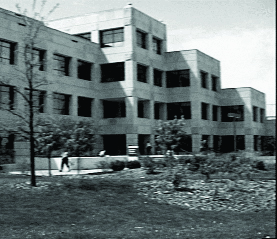
\includegraphics[alt={Picture of Durham you know}]{Images/dc5}

\caption{Durham Centre}
\label{mgraph}
\end{figure}

\subsubsection{Parts of the hypothesis}

Here one particular part of the hypothesis that is 
currently being explained is examined and particular
elements of that part are given careful scrutiny.

% Below \subsubsection
% Sectional commands: \paragraph and \subparagraph may also be used

\subsection{Second Hypothesis}

Here one particular hypothesis is explained in depth
and is examined in the light of current literature.

\subsubsection{Parts of the second hypothesis}

Here one particular part of the hypothesis that is 
currently being explained is examined and particular
elements of that part are given careful scrutiny.

\section{Criteria Review}

Here certain criteria are explained thus eventually
leading to a foregone conclusion.

% Chapter 5 from the standard thesis template
%   with a full page figure and a sideways table.
\chapter{SUMMARY AND DISCUSSION}

This is the opening paragraph to my thesis which
explains in general terms the concepts and hypothesis
which will be used in my thesis.

With more general information given here than really
necessary.

\section{Introduction}

Here initial concepts and conditions are explained and
several hypothesis are mentioned in brief.

Or graphically as seen in Figure~\ref{mgraph2}
it is certain that my hypothesis is true.

%\begin{figure}[p!] \centering

\begin{figure}[H] \centering % This goes with the package float comment this line out and use the previous one if you do not want to hold your position
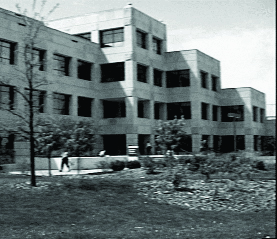
\includegraphics[alt={This is alt text}]{Images/dc5}

\isucaption{Durham Centre---  Another View}
\label{mgraph2}
\end{figure}

\subsection{Hypothesis}

Here one particular hypothesis is explained in depth
and is examined in the light of current literature.

As can be seen in Table~\ref{nothingelse} it is
truly obvious what I am saying is true.

%\addtocontents{lot}{\protect\newpage}

\begin{sidewaystable} \centering
\isucaption{This table shows almost nothing but is a
sideways table and takes up a whole page by itself}
\label{nothingelse}
% Use: \begin{tabular{|lcc|} to put table in a box
\begin{tabular}{lcc} \hline
\textbf{Element} & \textbf{Control} & \textbf{Experimental} \\ \hline
Moon Rings & 1.23 & 3.38 \\
Moon Tides & 2.26 & 3.12 \\
Moon Walk & 3.33 & 9.29 \\ \hline
\end{tabular}
\end{sidewaystable}

\subsubsection{Parts of the hypothesis}

Here one particular part of the hypothesis that is 
currently being explained is examined and particular
elements of that part are given careful scrutiny.

% Below \subsubsection
% Sectional commands: \paragraph and \subparagraph may also be used

%\addtocontents{toc}{\protect\newpage} %% Remove this if needed, this lines forces the lines of the TOC starting with the below sub-heading "Critical Review" to go to the next page. Remove this formatting line as it will be required only if you want to force a table of contents entry to the next page along with the other subsequent entries.

\subsection{Second Hypothesis}

Here one particular hypothesis is explained in depth
and is examined in the light of current literature.

\subsubsection{Parts of the second hypothesis}

Here one particular part of the hypothesis that is 
currently being explained is examined and particular
elements of that part are given careful scrutiny.

\section{Criteria Review}

Here certain criteria are explained thus eventually
leading to a foregone conclusion.

\section{Results And Discussion}

Here the results can be inserted


%\chapterbib

%\bibliographystyle{apa}
%\bibliography{Reference/mybib}

%% Rearranging the table of contents to show references before appendix
%\unappendixtitle
%\addcontentsline{toc}{chapter}{REFERENCES} %this line is to be included before the last chapter so that in toc it appears after the last chapter. If you want the reference to be the last entry of the toc, remove this line and in the biblio.tex file insert this line (or uncomment the line  )

\chapter*{BIBLIOGRAPHY}
\addToBibWithoutChapter{BIBLIOGRAPHY}
\printbibliography[heading=none]

%% Appendix1 file from standard thesis template

\appendixtitle 
\appendix


%% Use the following two lines for single appendix
%\unappendixtitle
%\singleappendixtitle

% Please note the appendix can be removed if the thesis does not require an overall appendix

\chapter{ADDITIONAL MATERIAL} 
This is now the same as any other chapter except that
all sectioning levels below the chapter level must begin
with the *-form of a sectioning command.

\section*{More stuff}

Supplemental material.

 
% % Instruction for single appendix check instruction in Appendix/appendix1.tex on top of the file
% % An example second appendix from the example thesis thesis.tex.
\chapter{STATISTICAL RESULTS}

This is now the same as any other chapter except that
all sectioning levels below the chapter level must begin
with the *-form of a sectioning command.

\section*{Supplemental Statistics}

More stuff.


\end{document}

% IMPORTANT NOTES
% TABLE OF CONTENTS :
% TOPIC 1:  If you need a page break follow the steps below
% step1
% check before which chapter in the table of contents you want a page break
% step 2
% go the folder "body". There open the chapter tex file that you noted needed page break in the table of contents..
% step 3
% insert  \addtocontents{toc}{\protect\newpage} before the first line i.e. before the line \chapter{RESULTS}.

%%%%%%%%%%%%%%%%%%%%%%%%%%%%
% \def\@makechapterhead#1{%   
% IN ORDER TO MAKE spacing changes in the title page got to the section in the isuthesis.cls file
% that starts with \long\def\maketitle{\begin{titlepage} and you can use options like
% singlespace (less spacing)
%singlespacing (comparitively more spacing almost like 2 spacing)
% onehalfspacing
%doublespacing (this is more spacing than the singlespacing above )
% more definitions on spacing can be found by going through the class file


% use \caption{} for all captions of figures and tables, where the captions are not too long.

% Use \caption[]{} with the square brackets for short caption of figure or table that goes into the list of tables and list of figures, and the curly brackets can have long captions which go with the figure/ table.

%%%%%% Using sub figures 
% %%% In preamble include : \usepackage{subfig}
% \begin{figure}[htbp]
% 	\centering
% 	\subfloat[first caption.\label{fig:2a}]{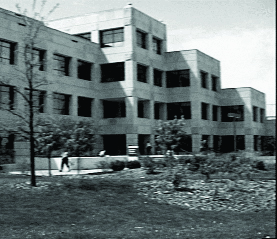
\includegraphics[width=0.2\textwidth]{Images/dc5.jpg}}\hfill
%     \subfloat[second caption.\label{fig:2b}] {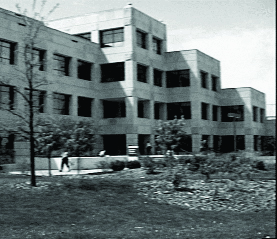
\includegraphics[width=0.2\textwidth]{Images/dc5.jpg}}\hfill
% 	\caption{Sub-figure test}
% 	\label{fig:subfigure-test}
% \end{figure}
